\documentclass[
  doc,
  longtable,
  nolmodern,
  notxfonts,
  notimes,
  colorlinks=true,linkcolor=blue,citecolor=blue,urlcolor=blue]{apa7}

\usepackage{amsmath}
\usepackage{amssymb}




\RequirePackage{longtable}
\RequirePackage{threeparttablex}

\makeatletter
\renewcommand{\paragraph}{\@startsection{paragraph}{4}{\parindent}%
	{0\baselineskip \@plus 0.2ex \@minus 0.2ex}%
	{-.5em}%
	{\normalfont\normalsize\bfseries\typesectitle}}

\renewcommand{\subparagraph}[1]{\@startsection{subparagraph}{5}{0.5em}%
	{0\baselineskip \@plus 0.2ex \@minus 0.2ex}%
	{-\z@\relax}%
	{\normalfont\normalsize\bfseries\itshape\hspace{\parindent}{#1}\textit{\addperi}}{\relax}}
\makeatother




\usepackage{longtable, booktabs, multirow, multicol, colortbl, hhline, caption, array, float, xpatch}
\setcounter{topnumber}{2}
\setcounter{bottomnumber}{2}
\setcounter{totalnumber}{4}
\renewcommand{\topfraction}{0.85}
\renewcommand{\bottomfraction}{0.85}
\renewcommand{\textfraction}{0.15}
\renewcommand{\floatpagefraction}{0.7}

\usepackage{tcolorbox}
\tcbuselibrary{listings,theorems, breakable, skins}
\usepackage{fontawesome5}

\definecolor{quarto-callout-color}{HTML}{909090}
\definecolor{quarto-callout-note-color}{HTML}{0758E5}
\definecolor{quarto-callout-important-color}{HTML}{CC1914}
\definecolor{quarto-callout-warning-color}{HTML}{EB9113}
\definecolor{quarto-callout-tip-color}{HTML}{00A047}
\definecolor{quarto-callout-caution-color}{HTML}{FC5300}
\definecolor{quarto-callout-color-frame}{HTML}{ACACAC}
\definecolor{quarto-callout-note-color-frame}{HTML}{4582EC}
\definecolor{quarto-callout-important-color-frame}{HTML}{D9534F}
\definecolor{quarto-callout-warning-color-frame}{HTML}{F0AD4E}
\definecolor{quarto-callout-tip-color-frame}{HTML}{02B875}
\definecolor{quarto-callout-caution-color-frame}{HTML}{FD7E14}

\newlength\Oldarrayrulewidth
\newlength\Oldtabcolsep


\usepackage{hyperref}




\providecommand{\tightlist}{%
  \setlength{\itemsep}{0pt}\setlength{\parskip}{0pt}}
\usepackage{longtable,booktabs,array}
\usepackage{calc} % for calculating minipage widths
% Correct order of tables after \paragraph or \subparagraph
\usepackage{etoolbox}
\makeatletter
\patchcmd\longtable{\par}{\if@noskipsec\mbox{}\fi\par}{}{}
\makeatother
% Allow footnotes in longtable head/foot
\IfFileExists{footnotehyper.sty}{\usepackage{footnotehyper}}{\usepackage{footnote}}
\makesavenoteenv{longtable}

\usepackage{graphicx}
\makeatletter
\def\maxwidth{\ifdim\Gin@nat@width>\linewidth\linewidth\else\Gin@nat@width\fi}
\def\maxheight{\ifdim\Gin@nat@height>\textheight\textheight\else\Gin@nat@height\fi}
\makeatother
% Scale images if necessary, so that they will not overflow the page
% margins by default, and it is still possible to overwrite the defaults
% using explicit options in \includegraphics[width, height, ...]{}
\setkeys{Gin}{width=\maxwidth,height=\maxheight,keepaspectratio}
% Set default figure placement to htbp
\makeatletter
\def\fps@figure{htbp}
\makeatother


% definitions for citeproc citations
\NewDocumentCommand\citeproctext{}{}
\NewDocumentCommand\citeproc{mm}{%
  \begingroup\def\citeproctext{#2}\cite{#1}\endgroup}
\makeatletter
 % allow citations to break across lines
 \let\@cite@ofmt\@firstofone
 % avoid brackets around text for \cite:
 \def\@biblabel#1{}
 \def\@cite#1#2{{#1\if@tempswa , #2\fi}}
\makeatother
\newlength{\cslhangindent}
\setlength{\cslhangindent}{1.5em}
\newlength{\csllabelwidth}
\setlength{\csllabelwidth}{3em}
\newenvironment{CSLReferences}[2] % #1 hanging-indent, #2 entry-spacing
 {\begin{list}{}{%
  \setlength{\itemindent}{0pt}
  \setlength{\leftmargin}{0pt}
  \setlength{\parsep}{0pt}
  % turn on hanging indent if param 1 is 1
  \ifodd #1
   \setlength{\leftmargin}{\cslhangindent}
   \setlength{\itemindent}{-1\cslhangindent}
  \fi
  % set entry spacing
  \setlength{\itemsep}{#2\baselineskip}}}
 {\end{list}}
\usepackage{calc}
\newcommand{\CSLBlock}[1]{\hfill\break\parbox[t]{\linewidth}{\strut\ignorespaces#1\strut}}
\newcommand{\CSLLeftMargin}[1]{\parbox[t]{\csllabelwidth}{\strut#1\strut}}
\newcommand{\CSLRightInline}[1]{\parbox[t]{\linewidth - \csllabelwidth}{\strut#1\strut}}
\newcommand{\CSLIndent}[1]{\hspace{\cslhangindent}#1}





\usepackage{newtx}

\defaultfontfeatures{Scale=MatchLowercase}
\defaultfontfeatures[\rmfamily]{Ligatures=TeX,Scale=1}





\title{Statistical Reporting Inconsistencies in Experimental
Linguistics}


\shorttitle{Statistical Inconsistencies}


\usepackage{etoolbox}








\authorsnames{Dara Leonard Jenssen Etemady,Timo B. Roettger}





\affiliation{
{Department of Linguistics \& Scandinavian Studies, University of Oslo}}




\leftheader{Etemady and Roettger}



\abstract{The present paper investigates the prevalence of statistical
reporting inconsistencies across articles in thirteen experimental
linguistics journals published between 2000 and 2023. Using the R
package ``Statcheck'', we retrieved 85,442 statistical test from 13,065
articles and assessed whether p-values were consistent with their test
statistic and degrees of freedom. Half of all articles (50\%) that used
null hypothesis significance testing contained at least one inconsistent
p-value. More than one in eight articles (13\%) contained an
inconsistency that may have affected the statistical conclusion. The
inconsistency rates were comparable across journals and seem stable over
publication years. We discuss possible reasons for this high rate and
offer actionable steps for authors, reviewers, and editors to remedy
this state-of-affairs.}

\keywords{statistics, Statcheck, reproducibility, null hypothesis
significance testing}

\authornote{\par{\addORCIDlink{Timo B. Roettger}{0000-0003-1400-2739}} 
\par{ }
\par{   The authors have no conflict of interest to
declare.   Conceptionalization, Methodology, Validation, Formal
Analysis, Review \& Editing of Manuscript, Data Curation - TBR. \& DLJE;
Software, Investigation - DLJE; Writing of Original Draft,
Visualization, Supervision - TBR. }
\par{Correspondence concerning this article should be addressed to Dara
Leonard Jenssen Etemady, Email: daraetemady@gmail.com}
}

\makeatletter
\let\endoldlt\endlongtable
\def\endlongtable{
\hline
\endoldlt
}
\makeatother

\urlstyle{same}



\usepackage{annotate-equations}
\makeatletter
\@ifpackageloaded{caption}{}{\usepackage{caption}}
\AtBeginDocument{%
\ifdefined\contentsname
  \renewcommand*\contentsname{Table of contents}
\else
  \newcommand\contentsname{Table of contents}
\fi
\ifdefined\listfigurename
  \renewcommand*\listfigurename{List of Figures}
\else
  \newcommand\listfigurename{List of Figures}
\fi
\ifdefined\listtablename
  \renewcommand*\listtablename{List of Tables}
\else
  \newcommand\listtablename{List of Tables}
\fi
\ifdefined\figurename
  \renewcommand*\figurename{Figure}
\else
  \newcommand\figurename{Figure}
\fi
\ifdefined\tablename
  \renewcommand*\tablename{Table}
\else
  \newcommand\tablename{Table}
\fi
}
\@ifpackageloaded{float}{}{\usepackage{float}}
\floatstyle{ruled}
\@ifundefined{c@chapter}{\newfloat{codelisting}{h}{lop}}{\newfloat{codelisting}{h}{lop}[chapter]}
\floatname{codelisting}{Listing}
\newcommand*\listoflistings{\listof{codelisting}{List of Listings}}
\makeatother
\makeatletter
\makeatother
\makeatletter
\@ifpackageloaded{caption}{}{\usepackage{caption}}
\@ifpackageloaded{subcaption}{}{\usepackage{subcaption}}
\makeatother

% From https://tex.stackexchange.com/a/645996/211326
%%% apa7 doesn't want to add appendix section titles in the toc
%%% let's make it do it
\makeatletter
\xpatchcmd{\appendix}
  {\par}
  {\addcontentsline{toc}{section}{\@currentlabelname}\par}
  {}{}
\makeatother

\begin{document}

\maketitle


\setcounter{secnumdepth}{5}

\setlength\LTleft{0pt}


\section{Introduction}\label{introduction}

What we know about human language and its cognitive underpinnings is
often informed by experimental data. Researchers test theoretical
predictions with their data using statistical tests. Depending on the
results of their tests, researchers make claims for or against
theoretical assumptions.\\
Since these tests play such an integral part in the argumentation
process of experimentalists, both the data these tests are based on and
the computational procedure of the tests itself should be error-free.
But humans are fallible; they make mistakes. We cannot avoid making
errors, but we can make them at least detectable. Transparent sharing
allows others to detect and correct human error.

In recent years, quantitative linguistics have seen repeated calls to
become more transparent and reproducible by sharing data and statistical
protocols, often under the banner of ``open science''
(\citeproc{ref-arvan2022reproducibility}{Arvan et al., 2022};
\citeproc{ref-laurinavichyute2022share}{Laurinavichyute et al., 2022};
\citeproc{ref-roettger2019researcher}{Roettger, 2019}). Despite these
calls, sharing of statistical protocols is still rather rare across the
language sciences (\citeproc{ref-bochynska2023reproducible}{Bochynska et
al., 2023}). If statistical procedures cannot be critically evaluated,
human errors might be left undetected and thus remain uncorrected in the
publication record. And if undetected errors affect the decision
procedure of the analysis, i.e.~whether a hypothesis is rejected or
accepted, these errors might lead to -at best- overconfident, -at worst-
false theoretical conclusions. The present paper will present evidence
that the published literature in experimental linguistics contains a
concerning amount of such statistical inconsitencies, a state of affairs
which warrants more rigorous data sharing practices.

\section{Statistal reporting
inconsistencies}\label{statistal-reporting-inconsistencies}

The null-hypothesis significance testing (NHST) framework is, to date,
the most dominant statistical framework that researchers use to test
hypotheses in the language sciences
(\citeproc{ref-sondereggera2024advancements}{Sonderegger \& Sóskuthy,
2024}). NHST tests are commonly reported in specific formats which
usually contain the name of the test (e.g.~F, t, χ2), a test statistic,
the degrees of freedom of that test (if applicable), and the p-value,
representing the probability of observing the data (or more extreme
data) given the null hypothesis (i.e.~given that the test statistic is
zero) (see example 1): ~

~

\begin{equation*}
  \tikzmarknode{node1}{(1) }
  \eqnmarkbox[gray]{node2}{F}
  \eqnmarkbox[orange]{node3}{(1,66)}
  \tikzmarknode{node4}{=}
  \eqnmarkbox[purple]{node5}{3.88}
  \tikzmarknode{node6}{, }
  \eqnmarkbox[blue]{node7}{p < .05}
\end{equation*}

\annotate[yshift=1em]{left}{node2}{name of test} 
\annotate[yshift=-1em]{below,left}{node3}{degrees of freedom} 
\annotate[yshift=1em]{right}{node5}{test statistic} 
\annotate[yshift=-1em]{below,right}{node7}{p-value}

~

Without access to the data and scripts, interested readers are left with
trusting the authors that the statistical analysis is run and reported
correctly. However, the three sets of indices in (1) have clearly
defined mathematical relationships and can thus be easily assessed for
consistency. For example, an F test with the specified degrees of
freedom and a test-statistic of 3.88 should result in a p-value of 0.053
which is larger, not smaller, than 0.05. Possible reasons for this
inconsistency are manifold: It could be a typo of the comparison sign,
i.e.~the authors meant to use \texttt{=} or \texttt{\textless{}} rather
than \texttt{\textgreater{}}. Additionally, any of the numbers could
contain a typo and sometimes an error might indicate erroneous rounding
(e.g.~0.057 being rounded down to 0.05). Without access to data and
scripts, it remains unclear to the reader what has caused this
inconsistency. Such inconsistencies can be particularly concerning if
the calculated p-value (here 0.057) and the reported p-values (here
\textless0.05) are not on the same side of the alpha threshold. In NHST,
p-values below a conventionalized alpha threshold, most commonly 0.05,
are interpreted as evidence that the data are sufficiently inconsistent
with the null hypothesis (``significant''). P-values above that
threshold are considered consistent with the null hypothesis and
practically lead to rejecting the alternative hypothesis
(``non-significant''). In (1) above, the reported p-value suggest a
significant result, the p-value derived from the degrees of freedom and
the test statistic suggest a non-significant result. In the following we
refer to these inconsistencies as ``decision inconsistencies''.

The consistency of these values can be automatically assessed if
statistical tests are reported in an unambiguous format. Recently, a
series of studies used such automatic assessments to evaluate the
prevalence of inconsistent statistical reporting in psychology
(\citeproc{ref-bakker2011mis}{Bakker \& Wicherts, 2011},
\citeproc{ref-bakker2014outlier}{2014};
\citeproc{ref-caperos2013consistency}{Caperos \& Pardo, 2013};
\citeproc{ref-claesen2023data}{Claesen et al., 2023};
\citeproc{ref-green2018statcheck}{Green et al., 2018};
\citeproc{ref-nuijten2016prevalence}{Nuijten et al., 2016};
\citeproc{ref-nuijten2020statcheck}{Nuijten \& Polanin, 2020};
\citeproc{ref-veldkamp2014statistical}{Veldkamp et al., 2014};
\citeproc{ref-wicherts2011willingness}{Wicherts et al., 2011}), medical
sciences (\citeproc{ref-garcia2004incongruence}{Garcı́a-Berthou \&
Alcaraz, 2004}; \citeproc{ref-van2023comparing}{Van Aert et al., 2023}),
psychiatry (\citeproc{ref-berle2007inconsistencies}{Berle \& Starcevic,
2007}), cyber security studies (\citeproc{ref-gross2021fidelity}{Groß,
2021}), technological education research
(\citeproc{ref-buckley2023estimating}{Buckley et al., 2023}), and
experimental philosophy (\citeproc{ref-colombo2018statistical}{Colombo
et al., 2018}). For example, looking at over 250,000 p-values published
in major psychology journals, Nuijten et al.
(\citeproc{ref-nuijten2016prevalence}{2016}) found that around 50\% of
the articles with statistical results contained at least one
inconsistency and around 13\% contained at least one decision
inconsistency. Other studies report on inconsistency rates between 4\%
and 14\%, with between 10\% and 63\% of articles containing at least one
inconsistency and between 3\% and 21\% contain at least one decision
consistency. These high inconsistency rates in other disciplines are
concerning and have led to a constructive dialog, resulting in
recommendations for best practice to either avoid inconsistencies or
make them more detectable.

To assess the prevalence of statistical reporting inconsistencies in
experimental linguistics, the present paper conceptually replicates
Nuijten et al. (\citeproc{ref-nuijten2016prevalence}{2016}) and assesses
p-values reported in thirteen experimental linguistic journals published
between 2000 and 2023. We explore whether the inconsistency rates differ
across journals, whether they have changed over the course of the last
23 years and whether there is evidence for bias in these
inconsistencies. We discuss the results and offer concrete
recommendations for authors, reviewers, and editors to tackle this
problem.

\section{Method}\label{method}

\subsection{Data availability
statement}\label{data-availability-statement}

All quantitative analyses were conducted using R Core Team
(\citeproc{ref-rmanual}{2025}). All derived data and corresponding R
scripts are available
\href{https://osf.io/gx3ub/?view_only=25957e06b5f449d6820b529eb0ae1937}{here}.

\subsection{Sample}\label{sample}

Focusing on experimental linguistic research, we used Kobrock and
Roettger (\citeproc{ref-kobrock2023assessing}{2023}) as a point of
departure who list 100 linguistic journals that had at least a hundred
articles published at the time of assessment (2021) and a high ratio of
articles containing the search string ``experiment*'' in title, abstract
and/or keywords. Out of these 100 journals, we selected all journals
with at least 10\% of articles containing the search string
``experiment*''. Out of the remaining 37 journals, we selected those
journals that urged APA formatting either in the main body of the text
or specifically regarding statistics in the author guidelines, resulting
in nine remaining journals. Moreover, to access the articles in .pdf
format, the articles had to be either accessible to us through our
library license, or open access, resulting in a final list of eight
journals: Applied Psycholinguistics (APS), Bilingualism: Language and
Cognition (BLC), Linguistic Approaches to Bilingualism (LAB), Language
and Speech (LaS), Language Learning and Techology (LLT), Journal of
Language and Social Psychology (LSP), Journal of Child Language (JCL),
and Studies in Second Language Acquisition (SLA). An anonymous reviewer
raised the justified concern that the resulting sample might not
represent the vast majority of work in experimental linguistics. To
address this concern, we additionally included those five journals that
have published the highest absolute number of experimental articles
(according to \citeproc{ref-kobrock2023assessing}{Kobrock \& Roettger,
2023}), regardless of whether they explicitly urge APA formatting or
not, resulting in the inclusion of the following psycholinguistic
outlets: Journal of Memory and Language (JML), Language, Cognition and
Neuroscience (LCN, former Language and Cognitive Processes), Journal of
Psycholinguistic Research (JPR), Journal Of Speech Language And Hearing
Research (SLH), and Brain and Language (BAL).

We included only original research articles within the publication years
of 2000-2023, excluding any book reviews, response articles,
commentaries, editorials, corrigenda, errata, advertisements, etc.

\subsection{Statcheck}\label{statcheck}

We used the R package Statcheck (Version 1.5.0,
\citeproc{ref-nuijten2023statcheck}{Nuijten \& Epskamp, 2024}) to
automatically detect statistical reporting inconsistencies. Statcheck
works as follows: After converting articles in pdf or html format to
plain text, Statcheck searches for specific strings that correspond to a
NHST result using regular expressions. That way, Statcheck can detect
results of t-tests, F-tests, Z-tests, χ2-tests, correlation tests, and
Q-tests as long as the test result fulfills three conditions: (a) the
test result is reported completely including the test statistic, the
degrees of freedom (if applicable), and the p-value; (b) the test result
is in the body of the text, i.e. Statcheck usually misses information in
tables; and (c) the test result is reported in American Psychological
Association style (\citeproc{ref-APA2020}{American Psychological
Association, 2020}). Given these constraints, Statcheck is estimated to
detect roughly 60\% of all reported NHST results
(\citeproc{ref-nuijten2016prevalence}{Nuijten et al., 2016}). Statcheck
uses the reported test statistic and degrees of freedom to recalculate
the p-value, compares the reported and recalculated p-value and, if
there is a mismatch, flags the test as containing an ``inconsistency.''
The algorithm takes into account that tests might have been performed as
one-tailed by identifying the search strings ``one-tailed,''
``one-sided,'' or ``directional'' in the body of the text. Moreover,
Statcheck considers p = .000 and p \textless{} .000 as inconsistent
because p-values of exactly zero are mathematically impossible and the
APA manual (\citeproc{ref-APA2020}{American Psychological Association,
2020}) advises to report very small p-values as p \textless{} .001.
Validity checks of Statcheck suggest that inter-rater reliability
between manual coding and Statcheck is high, i.e.~0.76 for
inconsistencies and 0.89 for decision inconsistencies
(\citeproc{ref-nuijten2016prevalence}{Nuijten et al., 2016}). The
overall accuracy of Statcheck is estimated to be between 96.2\% to
99.9\% (\citeproc{ref-nuijten2017validity}{Nuijten et al., 2017}). We
thus consider Statcheck a valid proxy of the prevalence of statistical
reporting inconsistencies.

Articles from Linguistic Approaches to Bilingualism spanned 2011-2023;
articles from Language, Cognition and Neuroscience spanned 2015-2023.
Statcheck could not parse 291 articles, likely related to issues with
rendering the Chi-Squared symbol being erroneously converted from .pdf
to .txt, resulting in some gaps in the coverage. This procedure resulted
in 13065 research articles which were submitted to analysis.

\subsection{Analysis and research
questions}\label{analysis-and-research-questions}

The aims of this study were explicitly exploratory and hypothesis
generating, thus analyses remain merely descriptive by reporting on the
proportion of articles/tests that are statistically (in)consistent. Our
investigation was set out to explore the following research questions:
(1) How prevalent are statistical inconsistencies (and decision
inconsistencies) in our sample? (see Section~\ref{sec-prevalent}) (2) Do
inconsistency rates vary across journals and/or their publication year?
(see Section~\ref{sec-stable}) And (3) is there evidence for bias,
i.e.~are processes that result in inconsistencies more likely to produce
lower p-values? (see Section~\ref{sec-bias})

\section{Results}\label{results}

\subsection{Inconsistencies are highly prevalent}\label{sec-prevalent}

The results are summarized in Table~\ref{tbl-summary}. Out of 13065
articles, 6484 articles contained statistical tests that Statcheck could
assess (50\%), amounting to 85442 assessable p-values. Interestingly,
the five journals that did not explicitly encourage APA formatting had
virtually identical rates of assessable articles compared to the
original sample. Overall, 11279 p-values were flagged as inconsistent
(13.2\%) out of which 1442 were considered decision inconsistencies
(1.7\%) (see Table~\ref{tbl-summary}).

\begin{table}

{\caption{{Number of eligible articles, assessable articles and results,
inconsistencies and decision inconsistencies across all journals.
(Applied Psycholinguistics (APS), Language and Brain (BAL),
Bilingualism: Language and Cognition (BLC), Journal of Memory and
Language (JML), Journal of Psycholinguistic Research (JPR), Linguistic
Approaches to Bilingualism (LAB), Language and Speech (LaS), Language
Cognition and Neuroscience (LCN, former Language and Cognitive
Processes), Language Learning and Techology (LLT), Journal of Language
and Social Psychology (LSP), Journal of Child Language (JCL), and
Studies in Second Language Acquisition (SLA), Journal Of Speech Language
And Hearing Research (SLH))}{\label{tbl-summary}}}}

\begin{longtable}[]{@{}
  >{\raggedright\arraybackslash}p{(\columnwidth - 10\tabcolsep) * \real{0.0755}}
  >{\raggedleft\arraybackslash}p{(\columnwidth - 10\tabcolsep) * \real{0.1698}}
  >{\raggedleft\arraybackslash}p{(\columnwidth - 10\tabcolsep) * \real{0.1887}}
  >{\raggedleft\arraybackslash}p{(\columnwidth - 10\tabcolsep) * \real{0.1792}}
  >{\raggedleft\arraybackslash}p{(\columnwidth - 10\tabcolsep) * \real{0.1509}}
  >{\raggedleft\arraybackslash}p{(\columnwidth - 10\tabcolsep) * \real{0.2358}}@{}}
\toprule\noalign{}
\begin{minipage}[b]{\linewidth}\raggedright
Journal
\end{minipage} & \begin{minipage}[b]{\linewidth}\raggedleft
eligible articles
\end{minipage} & \begin{minipage}[b]{\linewidth}\raggedleft
assessable articles
\end{minipage} & \begin{minipage}[b]{\linewidth}\raggedleft
assessable results
\end{minipage} & \begin{minipage}[b]{\linewidth}\raggedleft
inconsistencies
\end{minipage} & \begin{minipage}[b]{\linewidth}\raggedleft
decision inconsistencies
\end{minipage} \\
\midrule\noalign{}
\endhead
\bottomrule\noalign{}
\endlastfoot
APS & 953 & 690 & 9570 & 1447 & 198 \\
BAL & 2253 & 780 & 10344 & 1524 & 198 \\
BLC & 964 & 610 & 9093 & 1223 & 134 \\
JCL & 1109 & 529 & 6240 & 779 & 76 \\
JML & 1507 & 768 & 13236 & 1004 & 132 \\
JPR & 1137 & 534 & 5576 & 848 & 97 \\
LAB & 471 & 133 & 1719 & 239 & 25 \\
LCN & 751 & 397 & 5979 & 909 & 95 \\
LLT & 421 & 111 & 919 & 210 & 64 \\
LSP & 695 & 376 & 4320 & 449 & 68 \\
LaS & 597 & 362 & 4708 & 564 & 88 \\
SLA & 593 & 247 & 2954 & 476 & 66 \\
SLH & 1614 & 947 & 10784 & 1607 & 201 \\
Total & 13065 & 6484 & 85442 & 11279 & 1442 \\
\end{longtable}

\end{table}

\subsection{Inconsistencies are stable across journals and publication
year}\label{sec-stable}

The proportion of inconsistencies ranged from 8 to 23\% across journals
(1 to 7\% for decision inconsistencies) (see
Figure~\ref{fig-stacked-bar}). These rates appear to be stable across
year of publication (see Figure~\ref{fig-year-prop}). On average, 50\%
of assessable articles contained one or more inconsistencies (journals
range from 45 to 56\%) and 13\% contained one or more decision
inconsistencies (journals range from 11 to 17\%).

\begin{figure}[H]

\caption{\label{fig-stacked-bar}Proportion of articles containing at
least one inconsistency / decision inconsistency. (Applied
Psycholinguistics (APS), Language and Brain (BAL), Bilingualism:
Language and Cognition (BLC), Journal of Memory and Language (JML),
Journal of Psycholinguistic Research (JPR), Linguistic Approaches to
Bilingualism (LAB), Language and Speech (LaS), Language Cognition and
Neuroscience (LCN, former Language and Cognitive Processes), Language
Learning and Techology (LLT), Journal of Language and Social Psychology
(LSP), Journal of Child Language (JCL), and Studies in Second Language
Acquisition (SLA), Journal Of Speech Language And Hearing Research
(SLH))}

\centering{

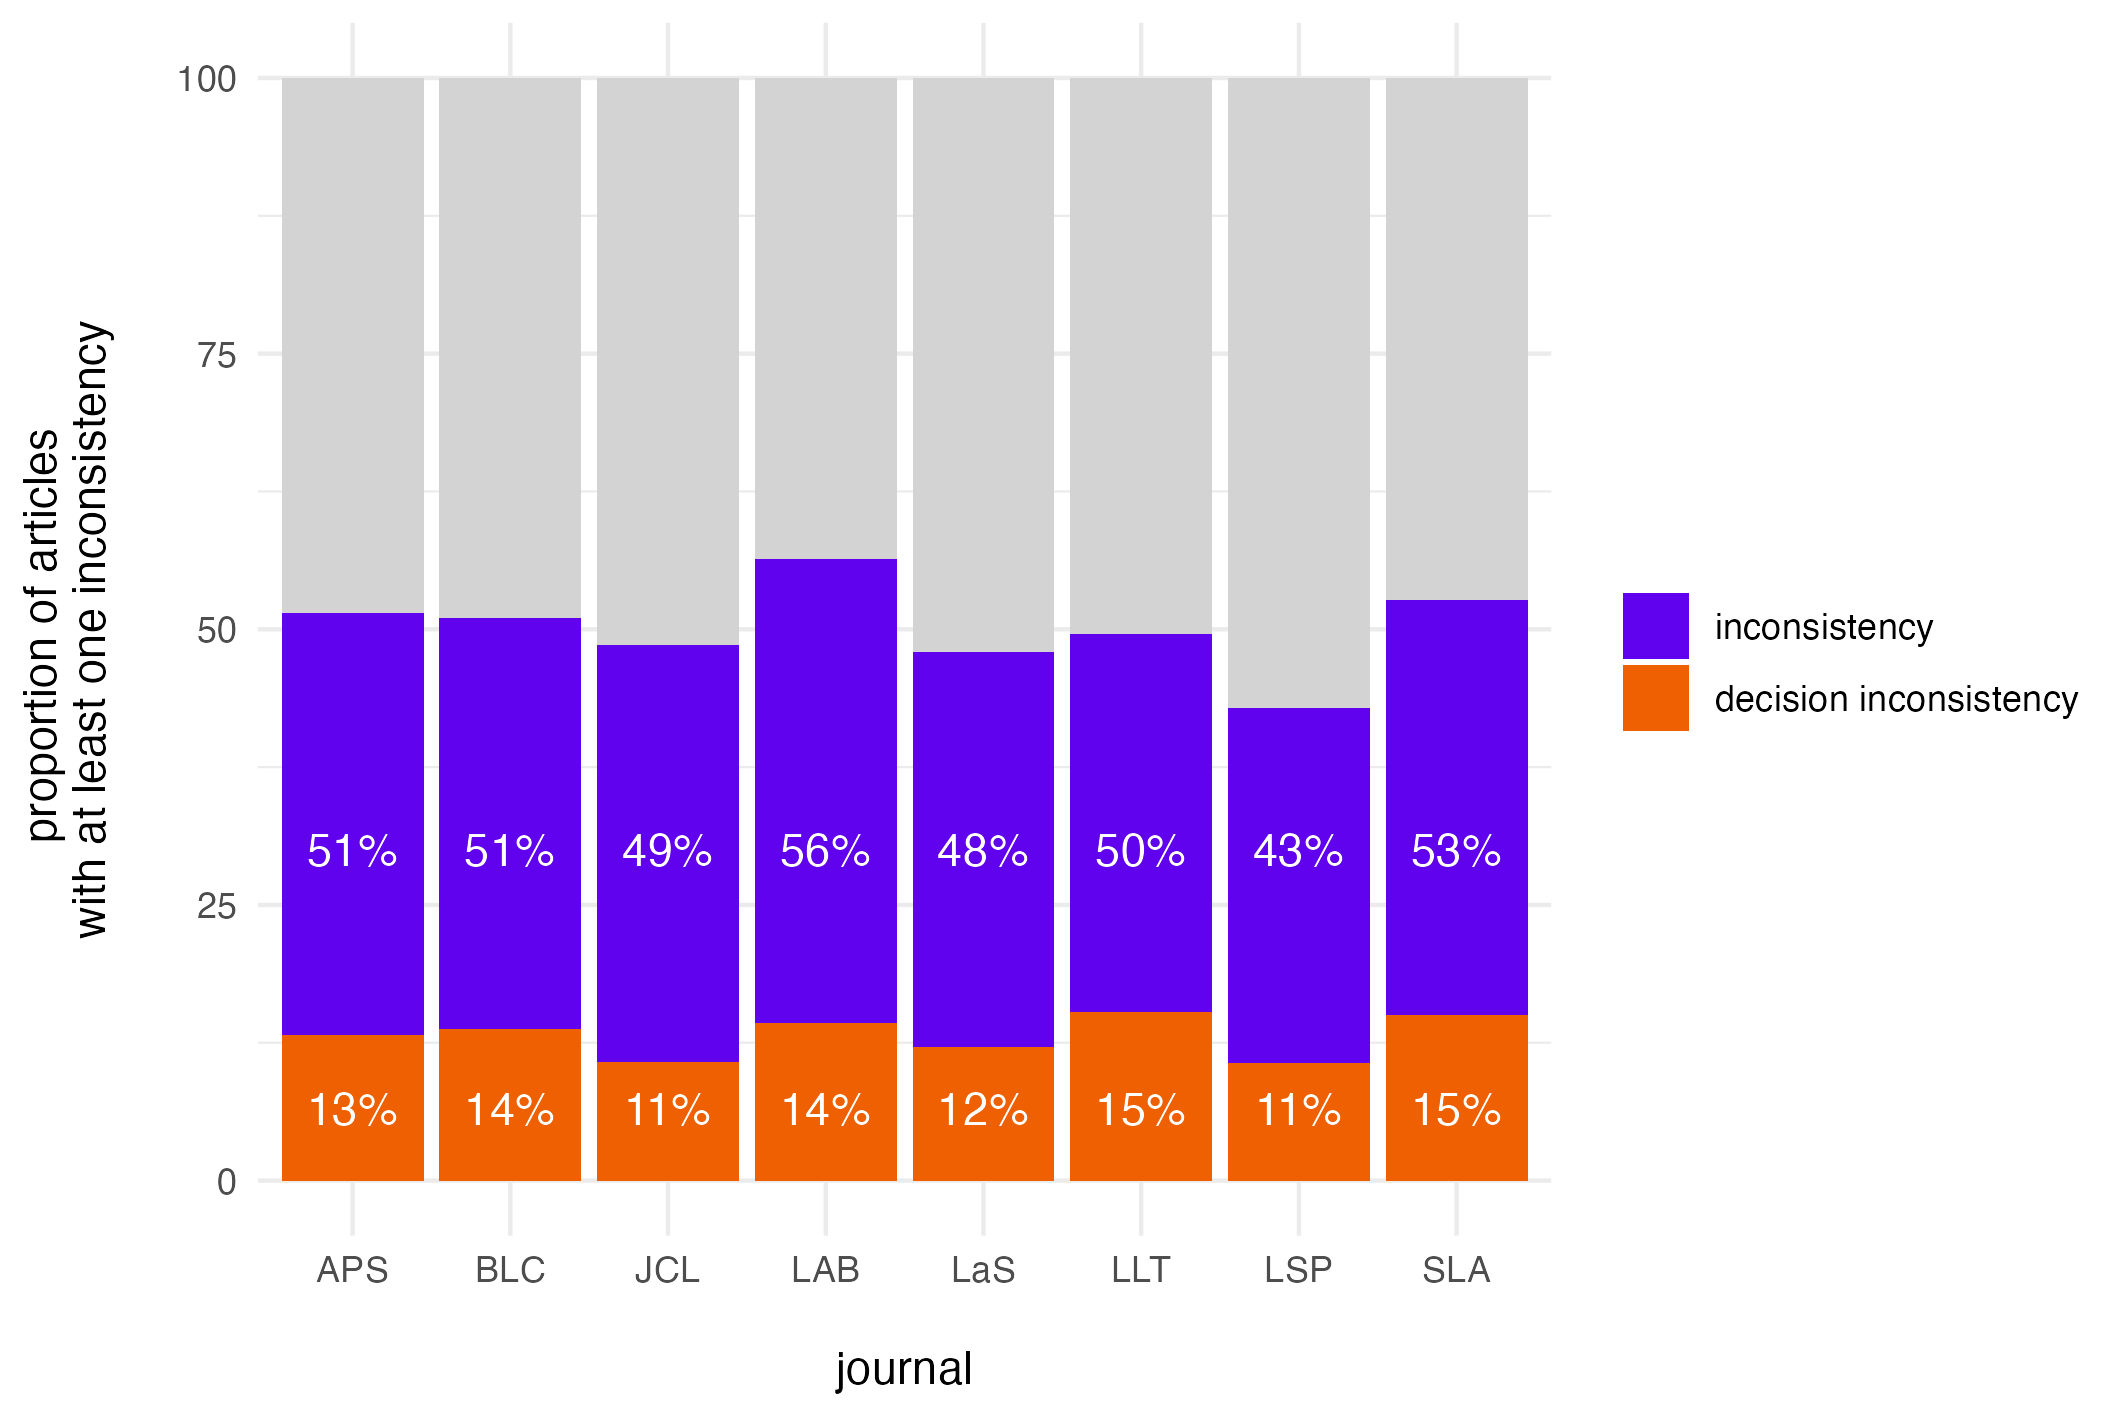
\includegraphics[width=1\textwidth,height=\textheight]{../plots/figure1.png}

}

\end{figure}%

\begin{figure}

\caption{\label{fig-year-prop}Proportion of inconsistencies / decision
inconsistencies across time overall (left panel) and split into journals
(right panel). (Applied Psycholinguistics (APS), Language and Brain
(BAL), Bilingualism: Language and Cognition (BLC), Journal of Memory and
Language (JML), Journal of Psycholinguistic Research (JPR), Linguistic
Approaches to Bilingualism (LAB), Language and Speech (LaS), Language
Cognition and Neuroscience (LCN, former Language and Cognitive
Processes), Language Learning and Techology (LLT), Journal of Language
and Social Psychology (LSP), Journal of Child Language (JCL), and
Studies in Second Language Acquisition (SLA), Journal Of Speech Language
And Hearing Research (SLH))}

\centering{

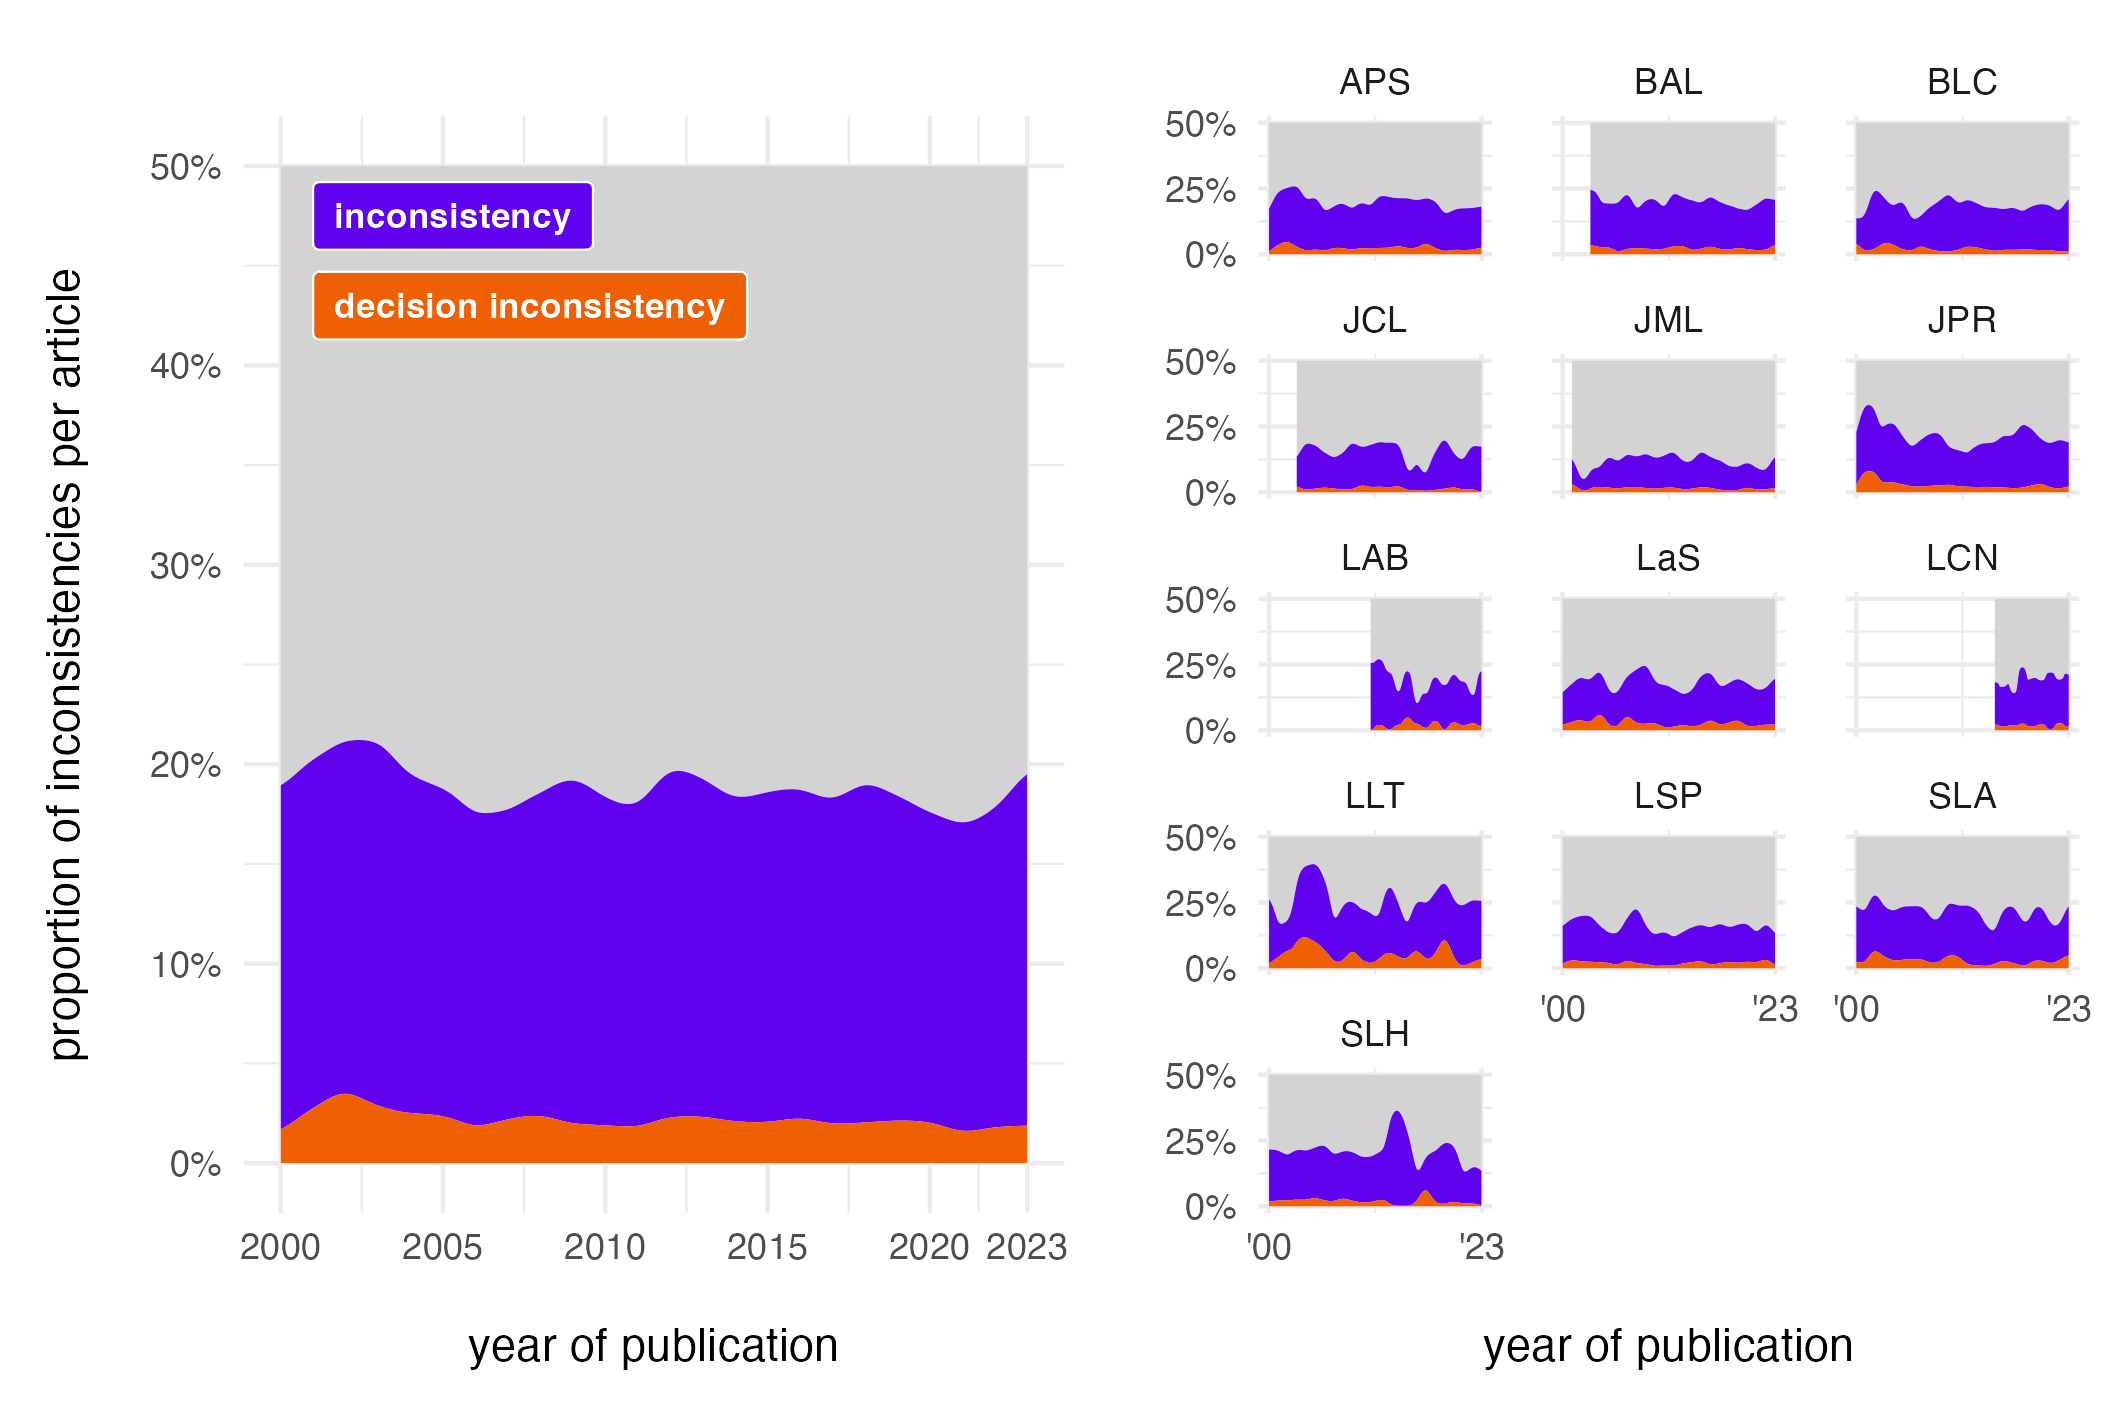
\includegraphics[width=1\textwidth,height=\textheight]{../plots/figure2.png}

}

\end{figure}%

\subsection{Inconsistencies appear biased but bias decreases over
time}\label{sec-bias}

If inconsistencies were bias-free, we would expect different types of
inconsistencies to be equally frequent. However, this is not the case.
Inconsistencies that report the p-value as being larger or smaller than
a reference value (e.g.~p \textgreater{} 0.05 or p \textless{} 0.05,
respectively) are not equally prevalent in the sample: There were 4.4\%
of inconsistencies with p being reported as larger than a reference but
7.1\% inconsistencies with p being reported as smaller than a reference.
So even if we assumed these inconsistencies were merely typos of the
comparison sign (e.g.~\textless{} instead of \textgreater),
inconsistencies that erroneously report the p-value to be smaller than a
reference value are more frequent than inconsistencies that erroneously
report the p-value to be larger than a reference value.

These biases are also reflected in decision inconsistencies. Of all
decision inconsistencies (n = 1442), 72\% represent cases in which a
reported significant result (p \textless{} 0.05) is recalculated as
non-significant (p \textgreater{} 0.05), i.e.~non-significant results
are more than twice as likely to be erroneously reported as significant
than the other way around. The latter pattern, however, seems to have
decreased over time. Reproducing Nuijten et al.
(\citeproc{ref-nuijten2016prevalence}{2016}), Figure~\ref{fig-scatter}
plots the development of the bias observed for decision inconsistencies
over time. The prevalence of decision inconsistencies in significant
p-values seems to have slightly decreased over the years, while the
prevalence of decision inconsistencies in non-significant p-values seems
to have slightly increased over the years.

\begin{figure}

\caption{\label{fig-scatter}Percentage of decision inconsistencies
falsely reporting significance (black) or non-significance (orange),
plotted across publication years.}

\centering{

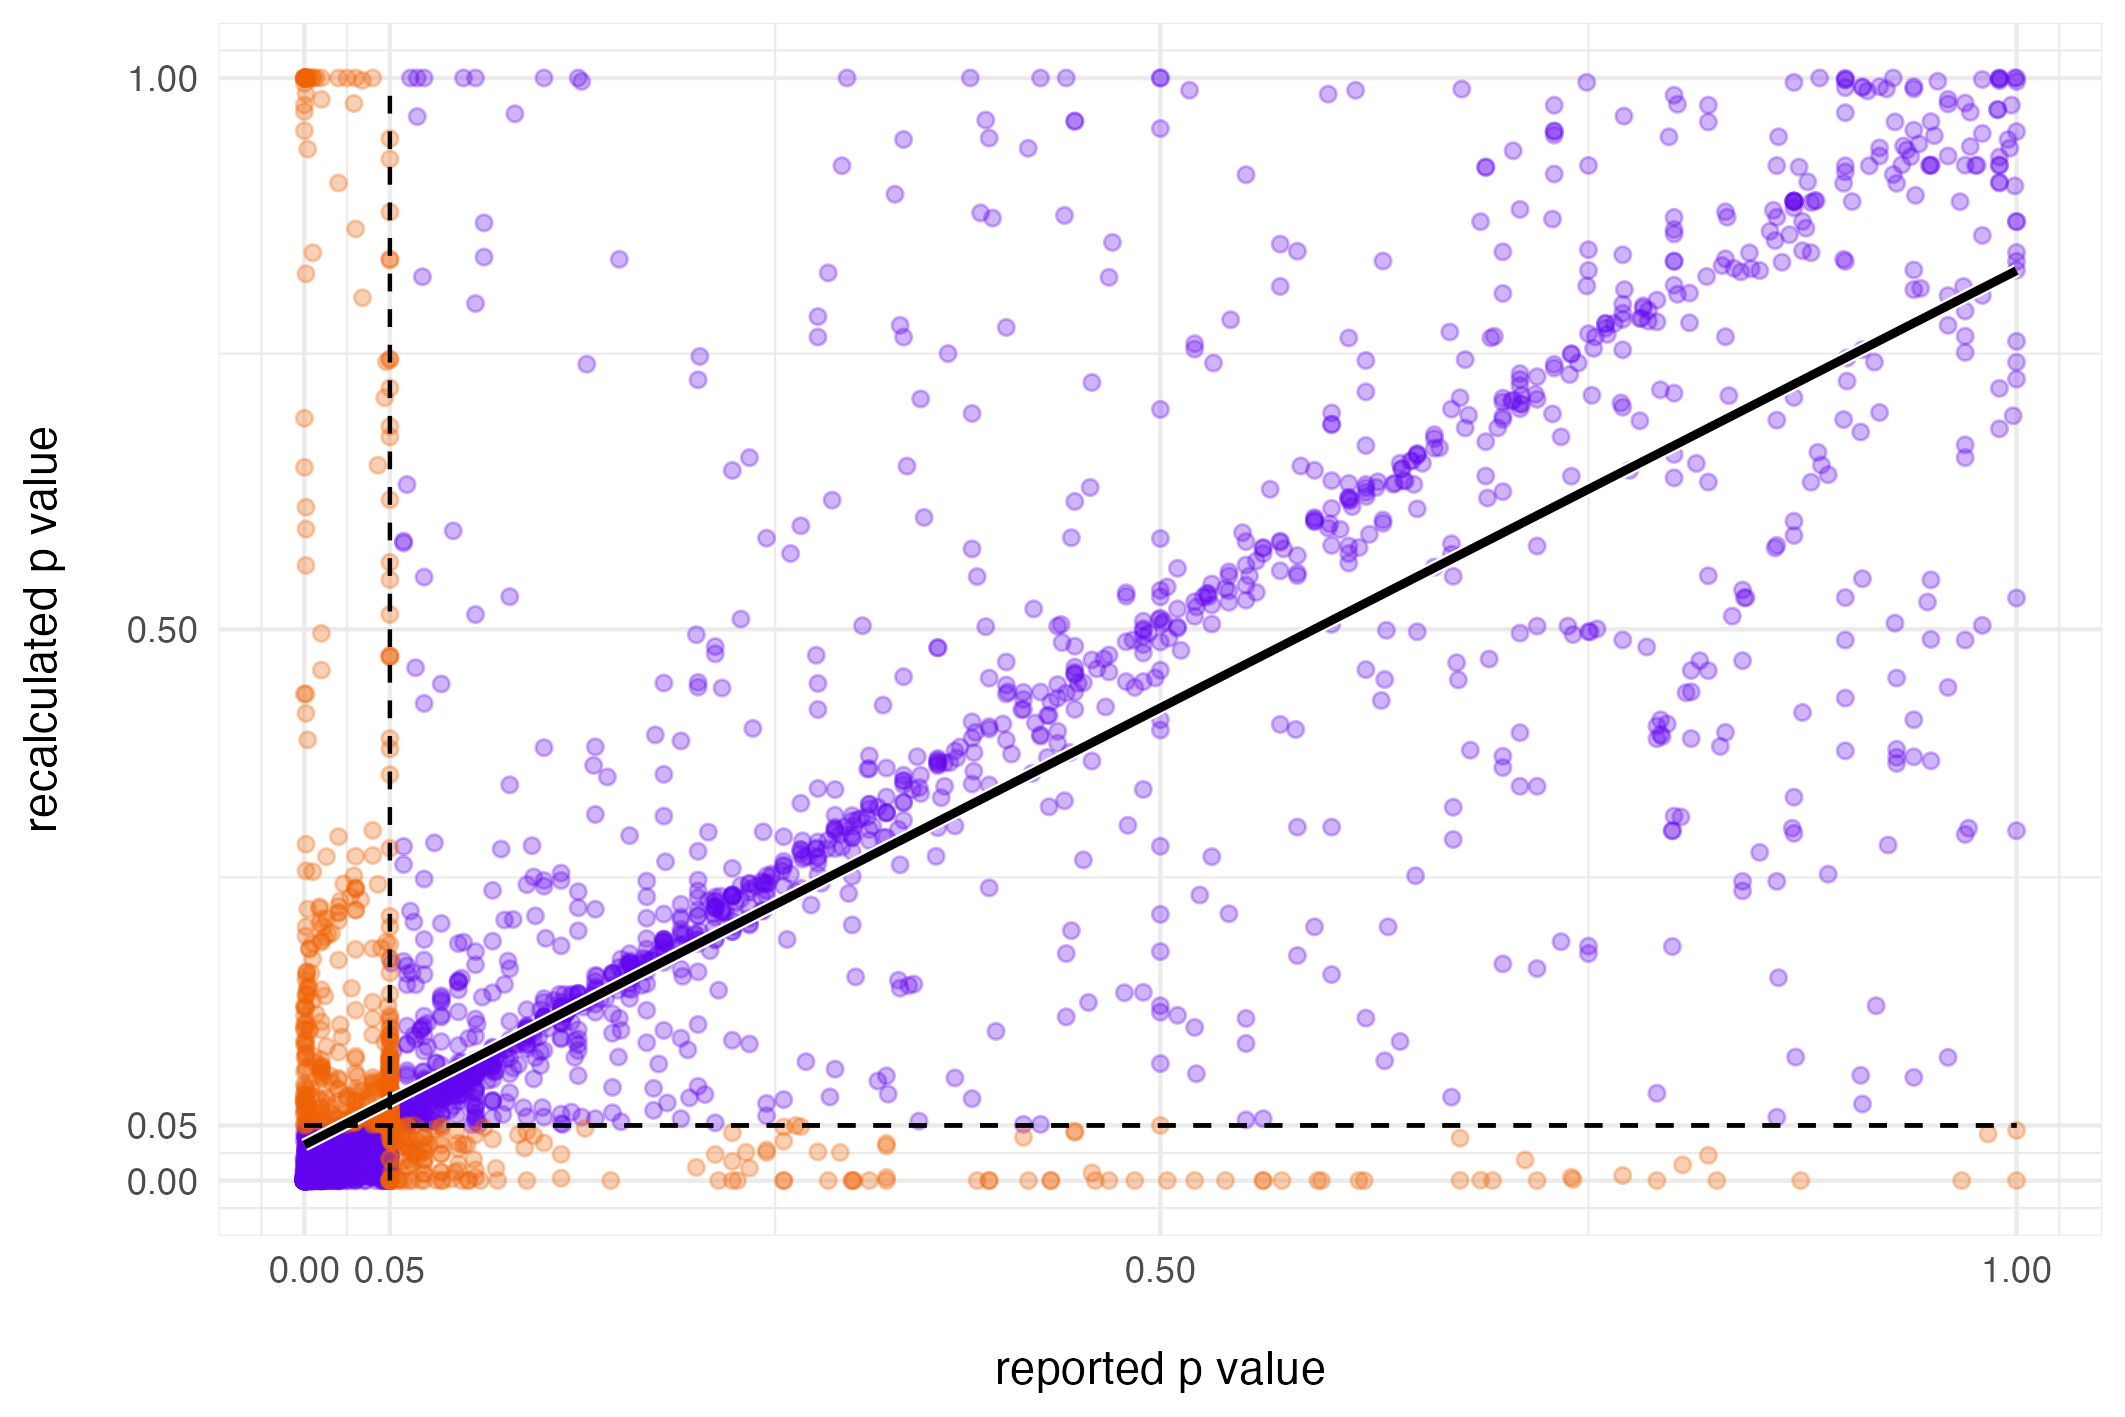
\includegraphics[width=0.8\textwidth,height=\textheight]{../plots/figure3.png}

}

\end{figure}%

\section{Discussion and
Recommendations}\label{discussion-and-recommendations}

\subsection{Statistical reporting inconsistencies are
prevalent}\label{statistical-reporting-inconsistencies-are-prevalent}

The present study found a large amount of statistical reporting
inconsistencies across a sample of 13065 experimental linguistic
articles, containing 85442 assessable p-values. 13.2\% of all p-values
were flagged as inconsistent and 1.7\% were flagged as decision
inconsistencies, i.e.~the reported p-value is on the opposite side of
the alpha threshold than the recalculated p-value. On average, 50\% of
assessable articles contained at least one inconsistency and 13\%
contained at least one decision inconsistency. The present examination
did not indicate any noticeable trend for inconsistency rates across
journals or publication year.

The present study can be considered a conceptual replication of previous
studies investigating statistical reporting inconsistency across
different disciplines (\citeproc{ref-bakker2011mis}{Bakker \& Wicherts,
2011}, \citeproc{ref-bakker2014outlier}{2014};
\citeproc{ref-caperos2013consistency}{Caperos \& Pardo, 2013};
\citeproc{ref-veldkamp2014statistical}{Veldkamp et al., 2014};
\citeproc{ref-wicherts2011willingness}{Wicherts et al., 2011}) and most
recent assessments using the automatic tool Statcheck
(\citeproc{ref-buckley2023estimating}{Buckley et al., 2023};
\citeproc{ref-colombo2018statistical}{Colombo et al., 2018};
\citeproc{ref-gross2021fidelity}{Groß, 2021};
\citeproc{ref-nuijten2016prevalence}{Nuijten et al., 2016}). The
discovered inconsistency rates fall in line with these studies that
report on rates between 4\% and 14\%, with between 10\% and 63\% of
articles containing at least one inconsistency. Moreover, the observed
rates of inconsistencies and decision inconsistencies are virtually
identical to rates reported on by Nuijten et al.
(\citeproc{ref-nuijten2016prevalence}{2016}) on the psychological
science literature.

Even if the prevalence of these inconsistencies could be largely
attributed to inconsequential typos or rounding errors (an assumption we
cannot test without access to the data), the sheer amount of these
inconsistencies that have made it through peer-review should concern us.
They are human errors. If such a substantial amount of errors is found
in plain site, the question naturally arises as to how many errors
during the data analysis itself remain undetected. We should ask
ourselves, if the tip of the iceberg is already so large, what is the
volume of the submerged iceberg?

Our results suggest biases as well. The prevalence of decision
inconsistencies was higher for p-values reported as significant than for
those reported as non-significant. These biases have been reported on
for other disciplines as well (\citeproc{ref-bakker2011mis}{Bakker \&
Wicherts, 2011}; \citeproc{ref-nuijten2016prevalence}{Nuijten et al.,
2016}). These skewed patterns could indicate a systematic bias in favor
of lower p-values in general and a bias towards significant results in
particular. Our data do not speak to the causes of these biases, but
possible reasons include the following:

First, researchers might intentionally round down p-values because they
think lower p-values are more convincing to reviewers and readers. This
practice has been admitted to by 1 in 5 surveyed psychological
researchers (\citeproc{ref-john2012measuring}{John et al., 2012}). Given
that a non-trivial amount of quantitative linguists have admitted to
commit questionable research practices (and even fraud)
(\citeproc{ref-isbell2022misconduct}{Isbell et al., 2022}), we cannot
exclude the possibility that some of the inconsistencies in our sample
were indeed intentional. It is our strong belief, however, that the
majority of inconsistencies are unintentional.

Second, researchers might scrutinize non-significant results more than
significant results or are less likely to double check significant
results than non-significant results because results that confirm their
hypothesis feed into their confirmation bias
(\citeproc{ref-nickerson1998confirmation}{Nickerson, 1998}). For
example, Fugelsang et al. (\citeproc{ref-fugelsang2004theory}{2004}) let
researchers evaluate data that are either consistent or inconsistent
with their prior expectations. They showed that when researchers
encounter results that are not in line with their expectations, they are
likely to blame the methodology while results that confirmed their
expectations were rarely critically scrutinized.

Third, the observed bias might merely be a reflection of publication
bias (\citeproc{ref-franco2014publication}{Franco et al., 2014};
\citeproc{ref-sterling1959publication}{Sterling, 1959}) with
(erroneously) reported significant p-values being more likely to be
published than (erroneously) reported non-significant ones. Publication
bias is a well established pattern in experimental linguistic research
with many recent meta analyses discussing possible evidence for it
(\citeproc{ref-isbilen2022statistical}{Isbilen \& Christiansen, 2022};
\citeproc{ref-lehtonen2018bilingualism}{Lehtonen et al., 2018};
\citeproc{ref-lu2024meta}{Lu et al., 2024}) For example, De Bruin et al.
(\citeproc{ref-de2015cognitive}{2015}) showed that studies with results
supporting the bilingual-advantage theory were most likely to be
published, while studies with results challenging the theory were
significantly less likely to be published.

Regardless of what possibly causes biases in the processes that generate
inconsistencies, our data also suggest a positive development. The over
proportional occurrence of decision inconsistencies for p-values
reported as significant has decreased over time.

\subsection{Limitations of our study}\label{limitations-of-our-study}

While we believe our work offers an important contribution to improving
statistical reporting practices in experimental linguistics, the present
assessment and the conclusions we can draw from them are limited. First,
our sample is limited to only a subset of experimental linguistic
journals. However, given the selection of journals and their standing in
the field, and given that the inconsistency rates of our study are not
only comparable to similar studies from other disciplines but also
relatively stable across journals and time, our findings should be
considered relevant for experimental linguistics at large.

Second, given the constraints on automatically detecting test
statistics, Statcheck misses reported values that either diverge from
APA reporting standards or are reported in tables. However,
inconsistency rates in our own sample have been shown to be similar for
results in APA format vs.~results that diverge from APA formatting
(\citeproc{ref-bakker2011mis}{Bakker \& Wicherts, 2011};
\citeproc{ref-nuijten2016prevalence}{Nuijten et al., 2016}).

Third, Statcheck slightly overestimates inconsistency rates, because it
might not accurately detect corrections for multiple comparisons
(\citeproc{ref-schmidt2017statcheck}{Schmidt, 2017}). Nuijten et al.
(\citeproc{ref-nuijten2017validity}{2017}), however, show that not only
were there only a small proportion of flagged inconsistencies related to
multiple comparisons, but also that these multiple comparisons
themselves were often erroneously reported. They conclude that
``{[}a{]}ny reporting inconsistencies associated with these tests and
corrections could not explain the high prevalence of reporting
inconsistencies'' (\citeproc{ref-nuijten2017validity}{Nuijten et al.,
2017, p. 27}).

More elaborate automatic tools for the extraction of statistical
information might allow for a more detailed and more accurate assessment
of statistical reporting in the future (e.g.
\citeproc{ref-kalmbach2023rule}{Kalmbach et al., 2023}). Despite its
limitations, Statcheck provides a rough proxy of true inconsistency
rates in the published literature and we hope the reader agrees that the
prevalence of inconsistencies is a state of affairs that should be
reflected upon.

\subsection{Recommendations for the
field}\label{recommendations-for-the-field}

There are concrete actionable steps the field of experimental
linguistics can take to reduce statistical reporting inconsistencies. In
order to avoid simple copy-and-paste errors related to working in two
separate programs for writing the manuscript and conducting the
statistical analysis, authors should consider `literate programming',
i.e.~an integration of analysis code and prose into a single, dynamic
document (\citeproc{ref-casillas2023opening}{Casillas et al., 2023};
\citeproc{ref-knuth1984literate}{Knuth, 1984}). Several implementations
of literate programming are freely available to researchers including
common R markdown files (Rmd) and Quarto markdown files (qmd). Literate
programming can ensure that values derived from the statistical analysis
are automatically integrated into the manuscript document, avoiding
errors that might happen during a manual transfer from one program to
the other.

Authors should generally engage in transparent and reproducible
practices that can reduce human error or at least make them detectable
by sharing their derived data (i.e.~the anonymized data table that was
analyzed) as well as a detailed description of their statistical
protocol, ideally in form of reproducible scripts. Sharing reproducible
analyses with reviewers allows the reviewers the reproduce the authors'
analyses, possibly detect errors or even inappropriate statistical
choices before publication, thus improving the quality and robustness of
the final product. Moreover, publicly sharing their analyses has
numerous benefits to the authors themselves beyond error detection: Open
data and materials can facilitate collaboration
(\citeproc{ref-boland2017ten}{Boland et al., 2017}), increase efficiency
and sustainability (\citeproc{ref-lowndes2017our}{Lowndes et al.,
2017}), and are cited more often
(\citeproc{ref-colavizza2020citation}{Colavizza et al., 2020}).

Reviewers can additionally check the statistical reporting consistency
in the manuscript by using tools such as Statcheck
(\citeproc{ref-nuijten2023statcheck}{Nuijten \& Epskamp, 2024},
http://statcheck.io) or p-checker
(\citeproc{ref-schonbrodt2015p}{Schönbrodt, 2015},
http://shinyapps.org/apps/p-checker/). Reviewers could consider
requesting data and scripts during peer review. Such requests might be
particularly justified when inconsistencies are apparent. Explicitly
requesting to share data might already instill additional care and
quality checks when authors prepare their materials, but also allows the
reviewers to carefully reproduce the results, and critically evaluate
all choices made in the statistical analysis
(\citeproc{ref-sakaluk2014analytic}{Sakaluk et al., 2014}). Recent
evidence suggest experimental linguistics are still characterized by a
pluralism of statistical approaches, even when trying to answer the same
research question (\citeproc{ref-coretta_multidimensional_2023}{Coretta
et al., 2023}). Some of these approaches might be more appropriate than
others (\citeproc{ref-sondereggera2024advancements}{Sonderegger \&
Sóskuthy, 2024}; \citeproc{ref-vasishth2023some}{Vasishth, 2023}), so
more thorough evaluations of how researchers arrive at their statistical
conclusions might elevate their analytical robustness. Moreover, a turn
towards inferential frameworks that do not focus on binary decision
procedures such as the null hypothesis significance testing framework,
might alleviate some of the biases we observed in the direction of
inconsistencies (\citeproc{ref-cumming2014new}{Cumming, 2014};
\citeproc{ref-vasishth2018statistical}{Vasishth et al., 2018}).

Journal editors could explicitly recommend consistency checks with
algorithms such as Statcheck during peer review, a practice that has
been taken up on by several journals from neighboring disciplines
(Psychological Science\footnote{http://www.psychologicalscience.org/publications/psychological\_science/ps-submissions;
  accessed on July 15, 2024.}, Advances in Methods and Practices in
Psychological Science\footnote{https://www.psychologicalscience.org/publications/ampps/ampps-submission-guidelines;
  accessed on on July 15, 2024.}, Stress \& Health Barber
(\citeproc{ref-barber2017meticulous}{2017})). Editors could also demand,
recommend or at least encourage data sharing for publication in their
journal. Data sharing policies have been shown to substantially increase
the reproducibility of analyses (e.g.,
\citeproc{ref-hardwicke2018data}{Hardwicke et al., 2018};
\citeproc{ref-laurinavichyute2022share}{Laurinavichyute et al., 2022})
and a number of linguistic journals have already implemented such
policies, including journals within our sample. Having said that, open
data policies which for example the Journal of Memory and Language
introduced in 2018 did not seem to have affected the proportion of
statistical inconsistencies after their introduction. The inconsistency
rates for JML (and other journals) were rather stable across time, so
open data alone might not resolve the issue without further changes to
the research eco-system.

Researchers make errors. Researchers have biases. This is who we are as
humans and there is not much we can do about our nature. Being aware of
this fact and how it might affect research might help us to make
possibly negative consequences detectable and preventable.

\section{References}\label{references}

\phantomsection\label{refs}
\begin{CSLReferences}{1}{0}
\bibitem[\citeproctext]{ref-APA2020}
American Psychological Association. (2020). \emph{Publication manual of
the {American Psychological Association}} (7th ed.). Author.
\url{https://doi.org/10.1037/0000173-000}

\bibitem[\citeproctext]{ref-arvan2022reproducibility}
Arvan, M., Pina, L., \& Parde, N. (2022). Reproducibility in
computational linguistics: Is source code enough? \emph{Proceedings of
the 2022 Conference on Empirical Methods in Natural Language
Processing}, 2350--2361.
\url{https://doi.org/10.18653/v1/2022.emnlp-main.150}

\bibitem[\citeproctext]{ref-bakker2011mis}
Bakker, M., \& Wicherts, J. M. (2011). The (mis) reporting of
statistical results in psychology journals. \emph{Behavior Research
Methods}, \emph{43}, 666--678.
\url{https://doi.org/10.3758/s13428-011-0089-5}

\bibitem[\citeproctext]{ref-bakker2014outlier}
Bakker, M., \& Wicherts, J. M. (2014). Outlier removal and the relation
with reporting errors and quality of psychological research. \emph{PloS
One}, \emph{9}(7), e103360.
\url{https://doi.org/10.1371/journal.pone.0103360}

\bibitem[\citeproctext]{ref-barber2017meticulous}
Barber, L. K. (2017). Meticulous manuscripts, messy results: Working
together for robust science reporting. \emph{Stress \& Health},
\emph{33}(2), 89--91. \url{https://doi.org/10.1002/smi.2756}

\bibitem[\citeproctext]{ref-berle2007inconsistencies}
Berle, D., \& Starcevic, V. (2007). Inconsistencies between reported
test statistics and p-values in two psychiatry journals.
\emph{International Journal of Methods in Psychiatric Research},
\emph{16}(4), 202--207. \url{https://doi.org/10.1002/mpr.225}

\bibitem[\citeproctext]{ref-bochynska2023reproducible}
Bochynska, A., Keeble, L., Halfacre, C., Casillas, J. V., Champagne,
I.-A., Chen, K., Röthlisberger, M., Buchanan, E. M., \& Roettger, T.
(2023). Reproducible research practices and transparency across
linguistics. \emph{Glossa Psycholinguistics}, \emph{2}(1).
\url{https://doi.org/10.5070/G6011239}

\bibitem[\citeproctext]{ref-boland2017ten}
Boland, M. R., Karczewski, K. J., \& Tatonetti, N. P. (2017). Ten simple
rules to enable multi-site collaborations through data sharing. In
\emph{PLoS computational biology} (1; Vol. 13, p. e1005278). Public
Library of Science San Francisco, CA USA.
\url{https://doi.org/10.1371/journal.pcbi.1005278}

\bibitem[\citeproctext]{ref-buckley2023estimating}
Buckley, J., Hyland, T., \& Seery, N. (2023). Estimating the
replicability of technology education research. \emph{International
Journal of Technology and Design Education}, \emph{33}(4), 1243--1264.
\url{https://doi.org/10.1007/s10798-022-09787-6}

\bibitem[\citeproctext]{ref-caperos2013consistency}
Caperos, J. M., \& Pardo, A. (2013). Consistency errors in p-values
reported in spanish psychology journals. \emph{Psicothema},
\emph{25}(3), 408--414. \url{https://doi.org/10.7334/psicothema2012.207}

\bibitem[\citeproctext]{ref-casillas2023opening}
Casillas, J. V., Constantin-Dureci, G., Rascón, I. A., Shao, J.,
Rodrı́guez, S. A., Gadamsetty, A., Minetti, A., Laungani, K., Thatcher,
J., Gardere, R.-T., et al. (2023). \emph{Opening open science to all:
Demystifying reproducibility and transparency practices in linguistic
research}. \url{https://doi.org/10.31234/osf.io/spz4w}

\bibitem[\citeproctext]{ref-claesen2023data}
Claesen, A., Vanpaemel, W., Maerten, A.-S., Verliefde, T., Tuerlinckx,
F., \& Heyman, T. (2023). Data sharing upon request and statistical
consistency errors in psychology: A replication of wicherts, bakker and
molenaar (2011). \emph{Plos One}, \emph{18}(4), e0284243.
\url{https://doi.org/10.1371/journal.pone.0284243}

\bibitem[\citeproctext]{ref-colavizza2020citation}
Colavizza, G., Hrynaszkiewicz, I., Staden, I., Whitaker, K., \&
McGillivray, B. (2020). The citation advantage of linking publications
to research data. \emph{PloS One}, \emph{15}(4), e0230416.
\url{https://doi.org/10.1371/journal.pone.0230416}

\bibitem[\citeproctext]{ref-colombo2018statistical}
Colombo, M., Duev, G., Nuijten, M. B., \& Sprenger, J. (2018).
Statistical reporting inconsistencies in experimental philosophy.
\emph{PloS One}, \emph{13}(4), e0194360.
\url{https://doi.org/10.1371/journal.pone.0194360}

\bibitem[\citeproctext]{ref-coretta_multidimensional_2023}
Coretta, S., Casillas, J. V., Roessig, S., Franke, M., Ahn, B.,
Al-Hoorie, A. H., Al-Tamimi, J., Alotaibi, N. E., AlShakhori, M. K.,
Altmiller, R. M., Arantes, P., Athanasopoulou, A., Baese-Berk, M. M.,
Bailey, G., Sangma, C. B. A., Beier, E. J., Benavides, G. M., Benker,
N., BensonMeyer, E. P., \ldots{} Roettger, T. B. (2023).
Multidimensional {Signals} and {Analytic} {Flexibility}: {Estimating}
{Degrees} of {Freedom} in {Human}-{Speech} {Analyses}. \emph{Advances in
Methods and Practices in Psychological Science}, \emph{6}(3),
25152459231162567. \url{https://doi.org/10.1177/25152459231162567}

\bibitem[\citeproctext]{ref-cumming2014new}
Cumming, G. (2014). The new statistics: Why and how. \emph{Psychological
Science}, \emph{25}(1), 7--29.

\bibitem[\citeproctext]{ref-de2015cognitive}
De Bruin, A., Treccani, B., \& Della Sala, S. (2015). Cognitive
advantage in bilingualism: An example of publication bias?
\emph{Psychological Science}, \emph{26}(1), 99--107.

\bibitem[\citeproctext]{ref-franco2014publication}
Franco, A., Malhotra, N., \& Simonovits, G. (2014). Publication bias in
the social sciences: Unlocking the file drawer. \emph{Science},
\emph{345}(6203), 1502--1505.
\url{https://doi.org/10.1126/science.1255484}

\bibitem[\citeproctext]{ref-fugelsang2004theory}
Fugelsang, J. A., Stein, C. B., Green, A. E., \& Dunbar, K. N. (2004).
Theory and data interactions of the scientific mind: Evidence from the
molecular and the cognitive laboratory. \emph{Canadian Journal of
Experimental Psychology/Revue Canadienne de Psychologie
Exp{é}rimentale}, \emph{58}(2), 86.
\url{https://doi.org/10.1037/h0085799}

\bibitem[\citeproctext]{ref-garcia2004incongruence}
Garcı́a-Berthou, E., \& Alcaraz, C. (2004). Incongruence between test
statistics and p values in medical papers. \emph{BMC Medical Research
Methodology}, \emph{4}, 1--5.
\url{https://doi.org/10.1186/1471-2288-4-13}

\bibitem[\citeproctext]{ref-green2018statcheck}
Green, C. D., Abbas, S., Belliveau, A., Beribisky, N., Davidson, I. J.,
DiGiovanni, J., Heidari, C., Martin, S. M., Oosenbrug, E., \&
Wainewright, L. M. (2018). Statcheck in canada: What proportion of CPA
journal articles contain errors in the reporting of p-values?
\emph{Canadian Psychology/Psychologie Canadienne}, \emph{59}(3), 203.
\url{https://doi.org/10.1037/cap0000139}

\bibitem[\citeproctext]{ref-gross2021fidelity}
Groß, T. (2021). Fidelity of statistical reporting in 10 years of cyber
security user studies. \emph{Socio-Technical Aspects in Security and
Trust: 9th International Workshop, STAST 2019, Luxembourg City,
Luxembourg, September 26, 2019, Revised Selected Papers 9}, 3--26.
\url{https://doi.org/10.1007/978-3-030-55958-8_1}

\bibitem[\citeproctext]{ref-hardwicke2018data}
Hardwicke, T. E., Mathur, M. B., MacDonald, K., Nilsonne, G., Banks, G.
C., Kidwell, M. C., Hofelich Mohr, A., Clayton, E., Yoon, E. J., Henry
Tessler, M., et al. (2018). Data availability, reusability, and analytic
reproducibility: Evaluating the impact of a mandatory open data policy
at the journal cognition. \emph{Royal Society Open Science},
\emph{5}(8), 180448. \url{https://doi.org/10.1098/rsos.180448}

\bibitem[\citeproctext]{ref-isbell2022misconduct}
Isbell, D. R., Brown, D., Chen, M., Derrick, D. J., Ghanem, R., Arvizu,
M. N. G., Schnur, E., Zhang, M., \& Plonsky, L. (2022). Misconduct and
questionable research practices: The ethics of quantitative data
handling and reporting in applied linguistics. \emph{The Modern Language
Journal}, \emph{106}(1), 172--195.
\url{https://doi.org/10.1111/modl.12760}

\bibitem[\citeproctext]{ref-isbilen2022statistical}
Isbilen, E. S., \& Christiansen, M. H. (2022). Statistical learning of
language: A meta-analysis into 25 years of research. \emph{Cognitive
Science}, \emph{46}(9), e13198.

\bibitem[\citeproctext]{ref-john2012measuring}
John, L. K., Loewenstein, G., \& Prelec, D. (2012). Measuring the
prevalence of questionable research practices with incentives for truth
telling. \emph{Psychological Science}, \emph{23}(5), 524--532.
\url{https://doi.org/10.1177/0956797611430953}

\bibitem[\citeproctext]{ref-kalmbach2023rule}
Kalmbach, T., Hoffmann, M., Lell, N., \& Scherp, A. (2023). On the
rule-based extraction of statistics reported in scientific papers.
\emph{International Conference on Applications of Natural Language to
Information Systems}, 326--338.
\url{https://doi.org/10.1007/978-3-031-35320-8_23}

\bibitem[\citeproctext]{ref-knuth1984literate}
Knuth, D. E. (1984). Literate programming. \emph{The Computer Journal},
\emph{27}(2), 97--111.

\bibitem[\citeproctext]{ref-kobrock2023assessing}
Kobrock, K., \& Roettger, T. (2023). Assessing the replication landscape
in experimental linguistics. \emph{Glossa Psycholinguistics},
\emph{2}(1), 1--28. \url{https://doi.org/10.5070/G6011135}

\bibitem[\citeproctext]{ref-laurinavichyute2022share}
Laurinavichyute, A., Yadav, H., \& Vasishth, S. (2022). Share the code,
not just the data: A case study of the reproducibility of articles
published in the journal of memory and language under the open data
policy. \emph{Journal of Memory and Language}, \emph{125}, 104332.
\url{https://doi.org/10.1016/j.jml.2022.104332}

\bibitem[\citeproctext]{ref-lehtonen2018bilingualism}
Lehtonen, M., Soveri, A., Laine, A., Järvenpää, J., De Bruin, A., \&
Antfolk, J. (2018). Is bilingualism associated with enhanced executive
functioning in adults? A meta-analytic review. \emph{Psychological
Bulletin}, \emph{144}(4), 394.

\bibitem[\citeproctext]{ref-lowndes2017our}
Lowndes, J. S. S., Best, B. D., Scarborough, C., Afflerbach, J. C.,
Frazier, M. R., O'Hara, C. C., Jiang, N., \& Halpern, B. S. (2017). Our
path to better science in less time using open data science tools.
\emph{Nature Ecology \& Evolution}, \emph{1}(6), 0160.
\url{https://doi.org/10.1038/s41559-017-0160}

\bibitem[\citeproctext]{ref-lu2024meta}
Lu, J., Frank, M., Degen, J., Lu, J., Frank, M. C., \& Degen, J. (2024).
A meta-analysis of syntactic satiation in extraction from islands.
\emph{Glossa Psycholinguistics}, \emph{3}(1).

\bibitem[\citeproctext]{ref-nickerson1998confirmation}
Nickerson, R. S. (1998). Confirmation bias: A ubiquitous phenomenon in
many guises. \emph{Review of General Psychology}, \emph{2}(2), 175--220.
\url{https://doi.org/10.1037/1089-2680.2.2.175}

\bibitem[\citeproctext]{ref-nuijten2017validity}
Nuijten, M. B., Assen, M. A. van, Hartgerink, C., Epskamp, S., \&
Wicherts, J. M. (2017). \emph{The validity of the tool {``statcheck''}
in discovering statistical reporting inconsistencies}.
\url{https://doi.org/10.31234/osf.io/tcxaj}

\bibitem[\citeproctext]{ref-nuijten2023statcheck}
Nuijten, M. B., \& Epskamp, S. (2024). \emph{Statcheck: Extract
statistics from articles and recompute p-values(1.5.0){[}r{]}}.

\bibitem[\citeproctext]{ref-nuijten2016prevalence}
Nuijten, M. B., Hartgerink, C. H., Van Assen, M. A., Epskamp, S., \&
Wicherts, J. M. (2016). The prevalence of statistical reporting errors
in psychology (1985--2013). \emph{Behavior Research Methods}, \emph{48},
1205--1226. \url{https://doi.org/10.5070/G6011135}

\bibitem[\citeproctext]{ref-nuijten2020statcheck}
Nuijten, M. B., \& Polanin, J. R. (2020). {``Statcheck''}: Automatically
detect statistical reporting inconsistencies to increase reproducibility
of meta-analyses. \emph{Research Synthesis Methods}, \emph{11}(5),
574--579.

\bibitem[\citeproctext]{ref-rmanual}
R Core Team. (2025). \emph{R: A language and environment for statistical
computing}. R Foundation for Statistical Computing.
\url{https://www.R-project.org/}

\bibitem[\citeproctext]{ref-roettger2019researcher}
Roettger, T. B. (2019). Researcher degrees of freedom in phonetic
research. \emph{Laboratory Phonology}, \emph{10}(1).
\url{https://doi.org/10.5334/labphon.147}

\bibitem[\citeproctext]{ref-sakaluk2014analytic}
Sakaluk, J., Williams, A., \& Biernat, M. (2014). Analytic review as a
solution to the misreporting of statistical results in psychological
science. \emph{Perspectives on Psychological Science}, \emph{9}(6),
652--660. \url{https://doi.org/10.1177/1745691614549257}

\bibitem[\citeproctext]{ref-schmidt2017statcheck}
Schmidt, T. (2017). \emph{Statcheck does not work: All the numbers.
Reply to nuijten et al.(2017)}.
\url{https://doi.org/10.31234/osf.io/hr6qy}

\bibitem[\citeproctext]{ref-schonbrodt2015p}
Schönbrodt, F. D. (2015). \emph{P-checker: One-for-all p-value
analyzer}. \url{http://shinyapps.org/apps/p-checker/}.

\bibitem[\citeproctext]{ref-sondereggera2024advancements}
Sonderegger, M., \& Sóskuthy, M. (2024). \emph{Advancements of phonetics
in the 21st century: Quantitative data analysis}.
\url{https://doi.org/10.31234/osf.io/mc6a9}

\bibitem[\citeproctext]{ref-sterling1959publication}
Sterling, T. D. (1959). Publication decisions and their possible effects
on inferences drawn from tests of significance---or vice versa.
\emph{Journal of the American Statistical Association}, \emph{54}(285),
30--34. \url{https://doi.org/10.2307/2282137}

\bibitem[\citeproctext]{ref-van2023comparing}
Van Aert, R. C., Nuijten, M. B., Olsson-Collentine, A., Stoevenbelt, A.
H., Van Den Akker, O. R., Klein, R. A., \& Wicherts, J. M. (2023).
Comparing the prevalence of statistical reporting inconsistencies in
COVID-19 preprints and matched controls: A registered report.
\emph{Royal Society Open Science}, \emph{10}(8), 202326.
\url{https://doi.org/10.1098/rsos.202326}

\bibitem[\citeproctext]{ref-vasishth2023some}
Vasishth, S. (2023). Some right ways to analyze (psycho) linguistic
data. \emph{Annual Review of Linguistics}, \emph{9}(1), 273--291.
\url{https://doi.org/10.1146/annurev-linguistics-031220-010345}

\bibitem[\citeproctext]{ref-vasishth2018statistical}
Vasishth, S., Mertzen, D., Jäger, L. A., \& Gelman, A. (2018). The
statistical significance filter leads to overoptimistic expectations of
replicability. \emph{Journal of Memory and Language}, \emph{103},
151--175.

\bibitem[\citeproctext]{ref-veldkamp2014statistical}
Veldkamp, C. L., Nuijten, M. B., Dominguez-Alvarez, L., Van Assen, M.
A., \& Wicherts, J. M. (2014). Statistical reporting errors and
collaboration on statistical analyses in psychological science.
\emph{PloS One}, \emph{9}(12), e114876.
\url{https://doi.org/10.1371/journal.pone.0114876}

\bibitem[\citeproctext]{ref-wicherts2011willingness}
Wicherts, J. M., Bakker, M., \& Molenaar, D. (2011). Willingness to
share research data is related to the strength of the evidence and the
quality of reporting of statistical results. \emph{PloS One},
\emph{6}(11), e26828. \url{https://doi.org/10.1371/journal.pone.0026828}

\end{CSLReferences}






\end{document}
